\chapter*{Acknowledgments}
\addcontentsline{toc}{chapter}{Acknowledgments}
Going through this PhD has truely being a remarkable experience.  It has taught me many valuable lessons, 
but the most important one is to not get intimidated by a hard problem.  During this journey, I 
was fortunate to have guidance and support from many people. 	


First and foremost, this thesis could not have been possible without the support of my supervisor, Dirk Pattinson. I really 
admire this abilities and intuition to make sure that I stay clear from many dead ends. Moreover, 
I thank him for patiently answering my stupid questions happily and guiding me towards the right 
answer by asking the right questions. My only wish to be researcher like 
him and incorporate more of his qualities, but I am less optimistic about my chance. 

I also want to thank my dog, Turbo, whom I can talk for hours, and he never judged me. He 
would patiently listen to my proofs
and ideas about electronic voting with occasionally barking at me if he was bored of listening. 
His listening helped me in developing my ideas more better. 
Turbo truly made my PhD a breeze, and I never felt pressure of PhD when I was with him. Thank you
Turbo, and you are the best dog. 
%\begin{figure}[h]
%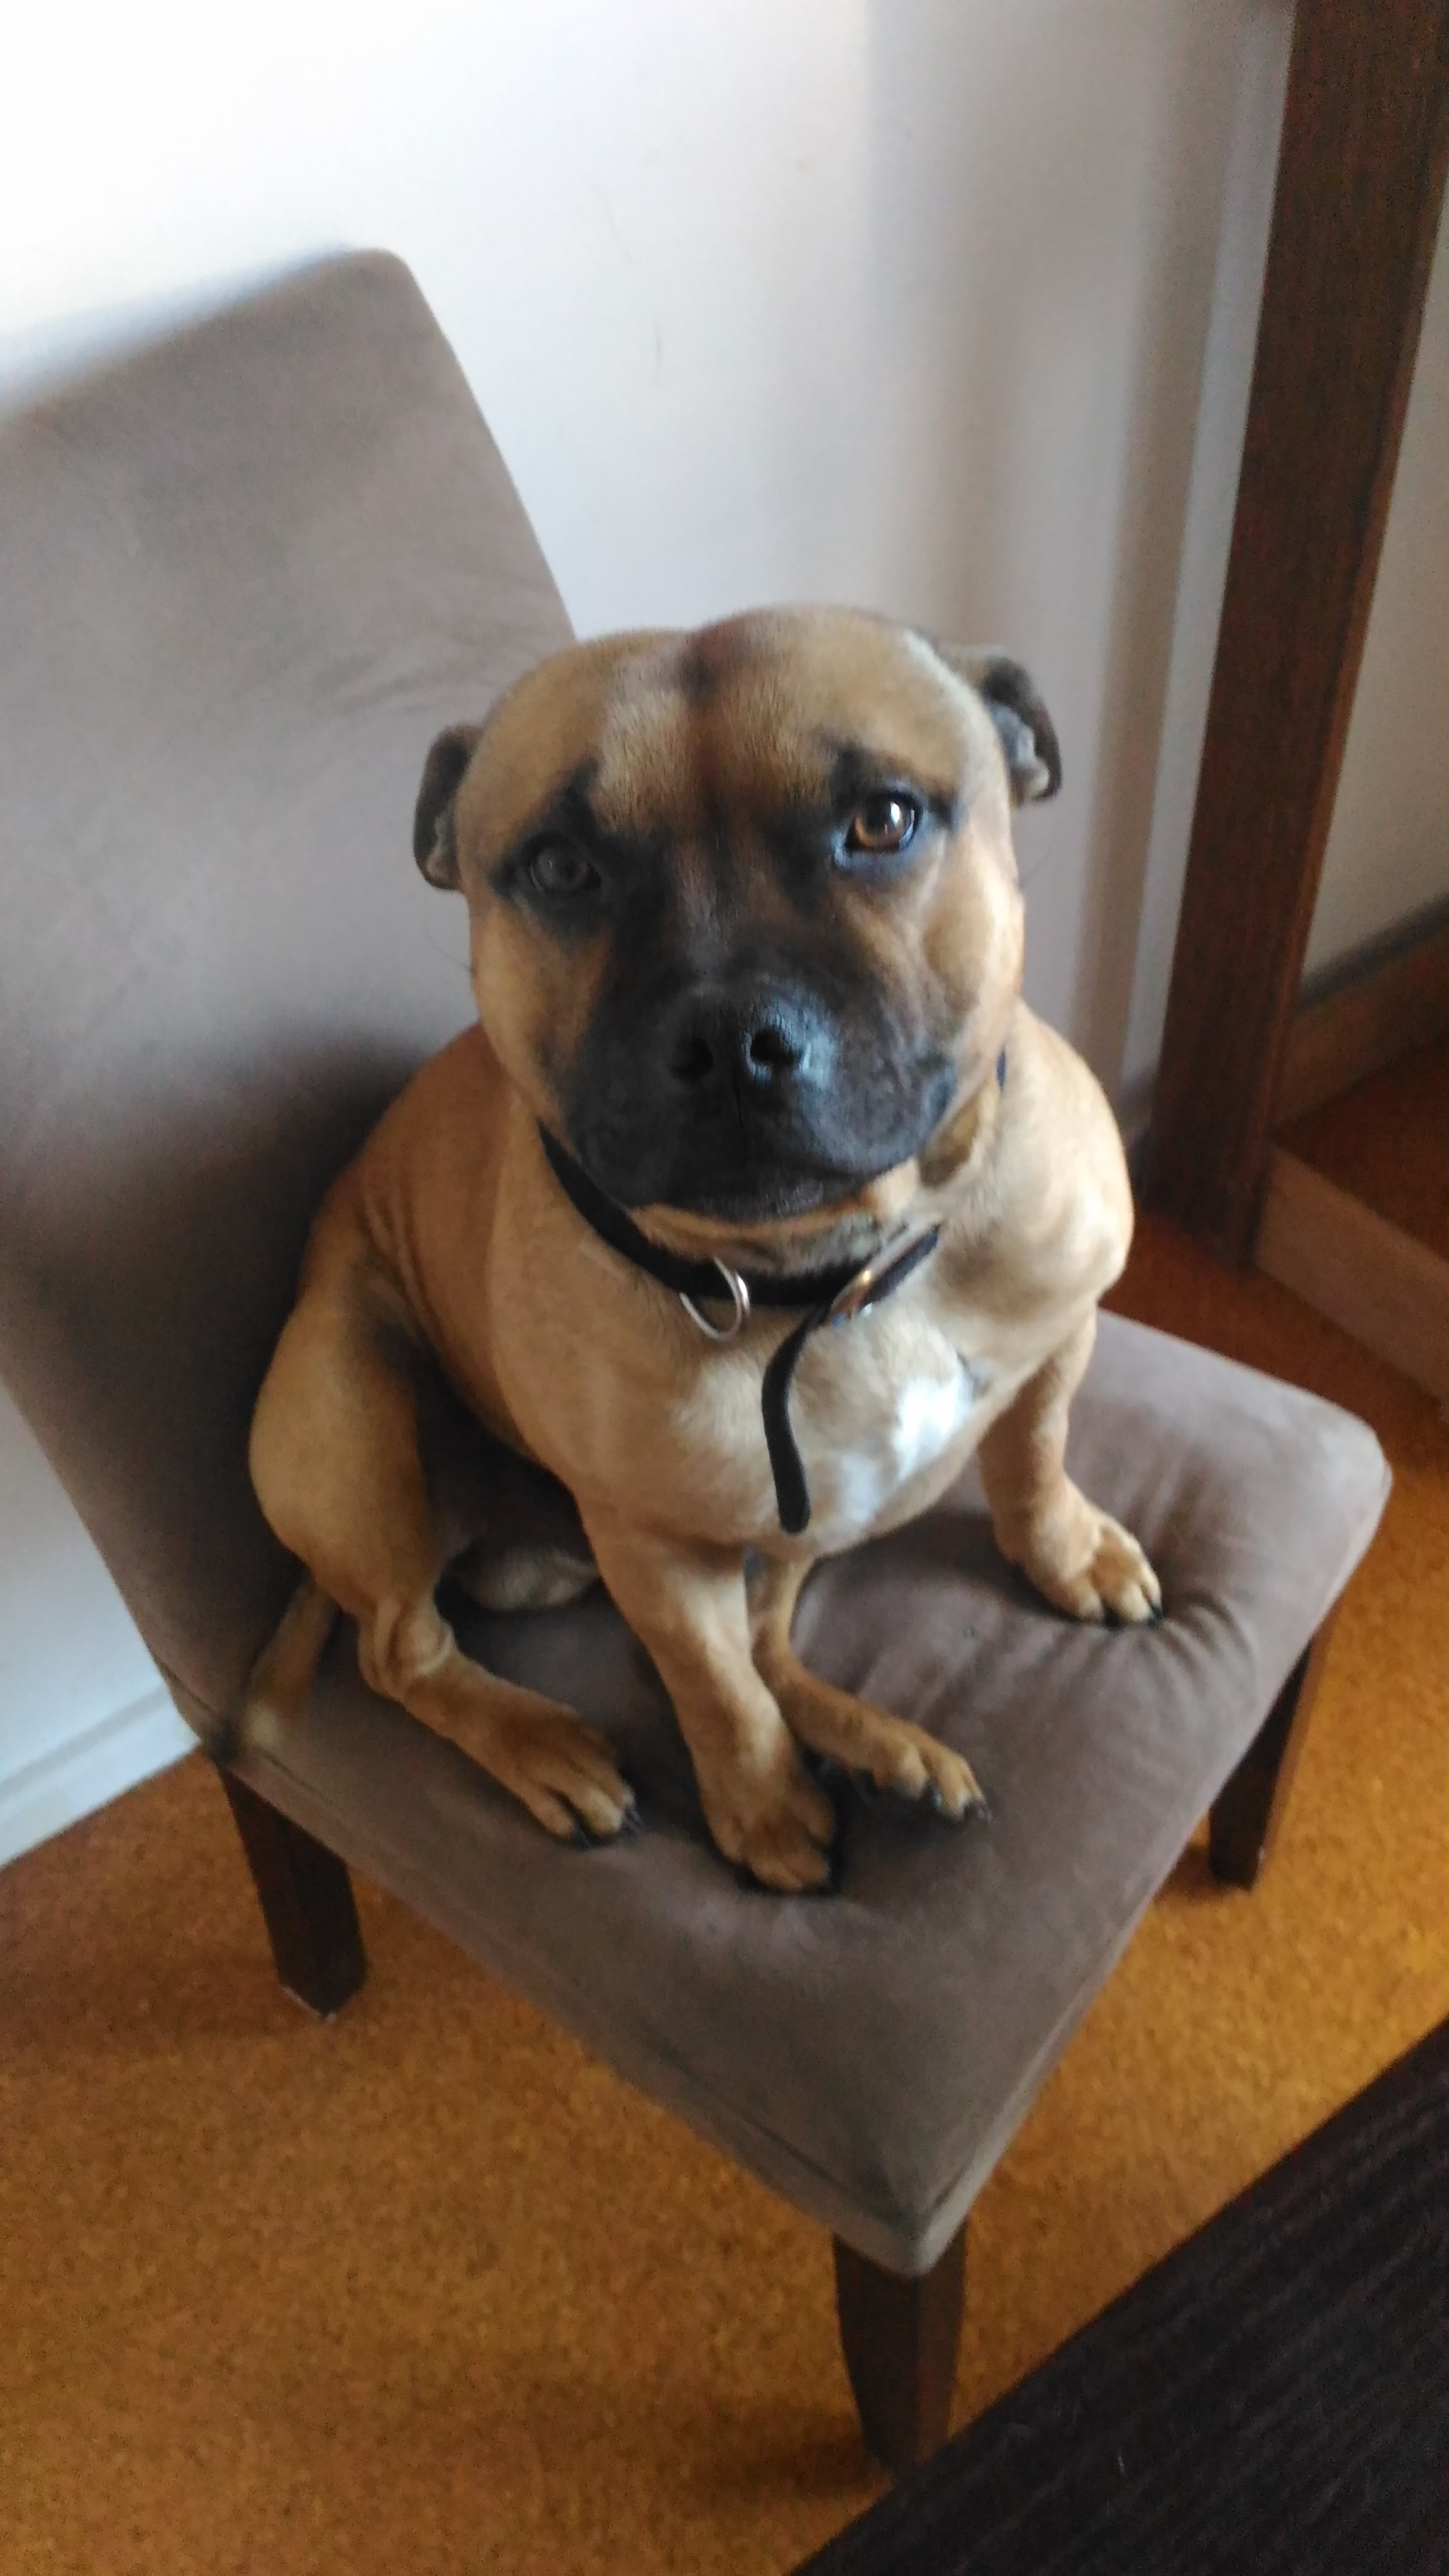
\includegraphics[width=8cm]{figs/turbo.jpg}
%\end{figure}
%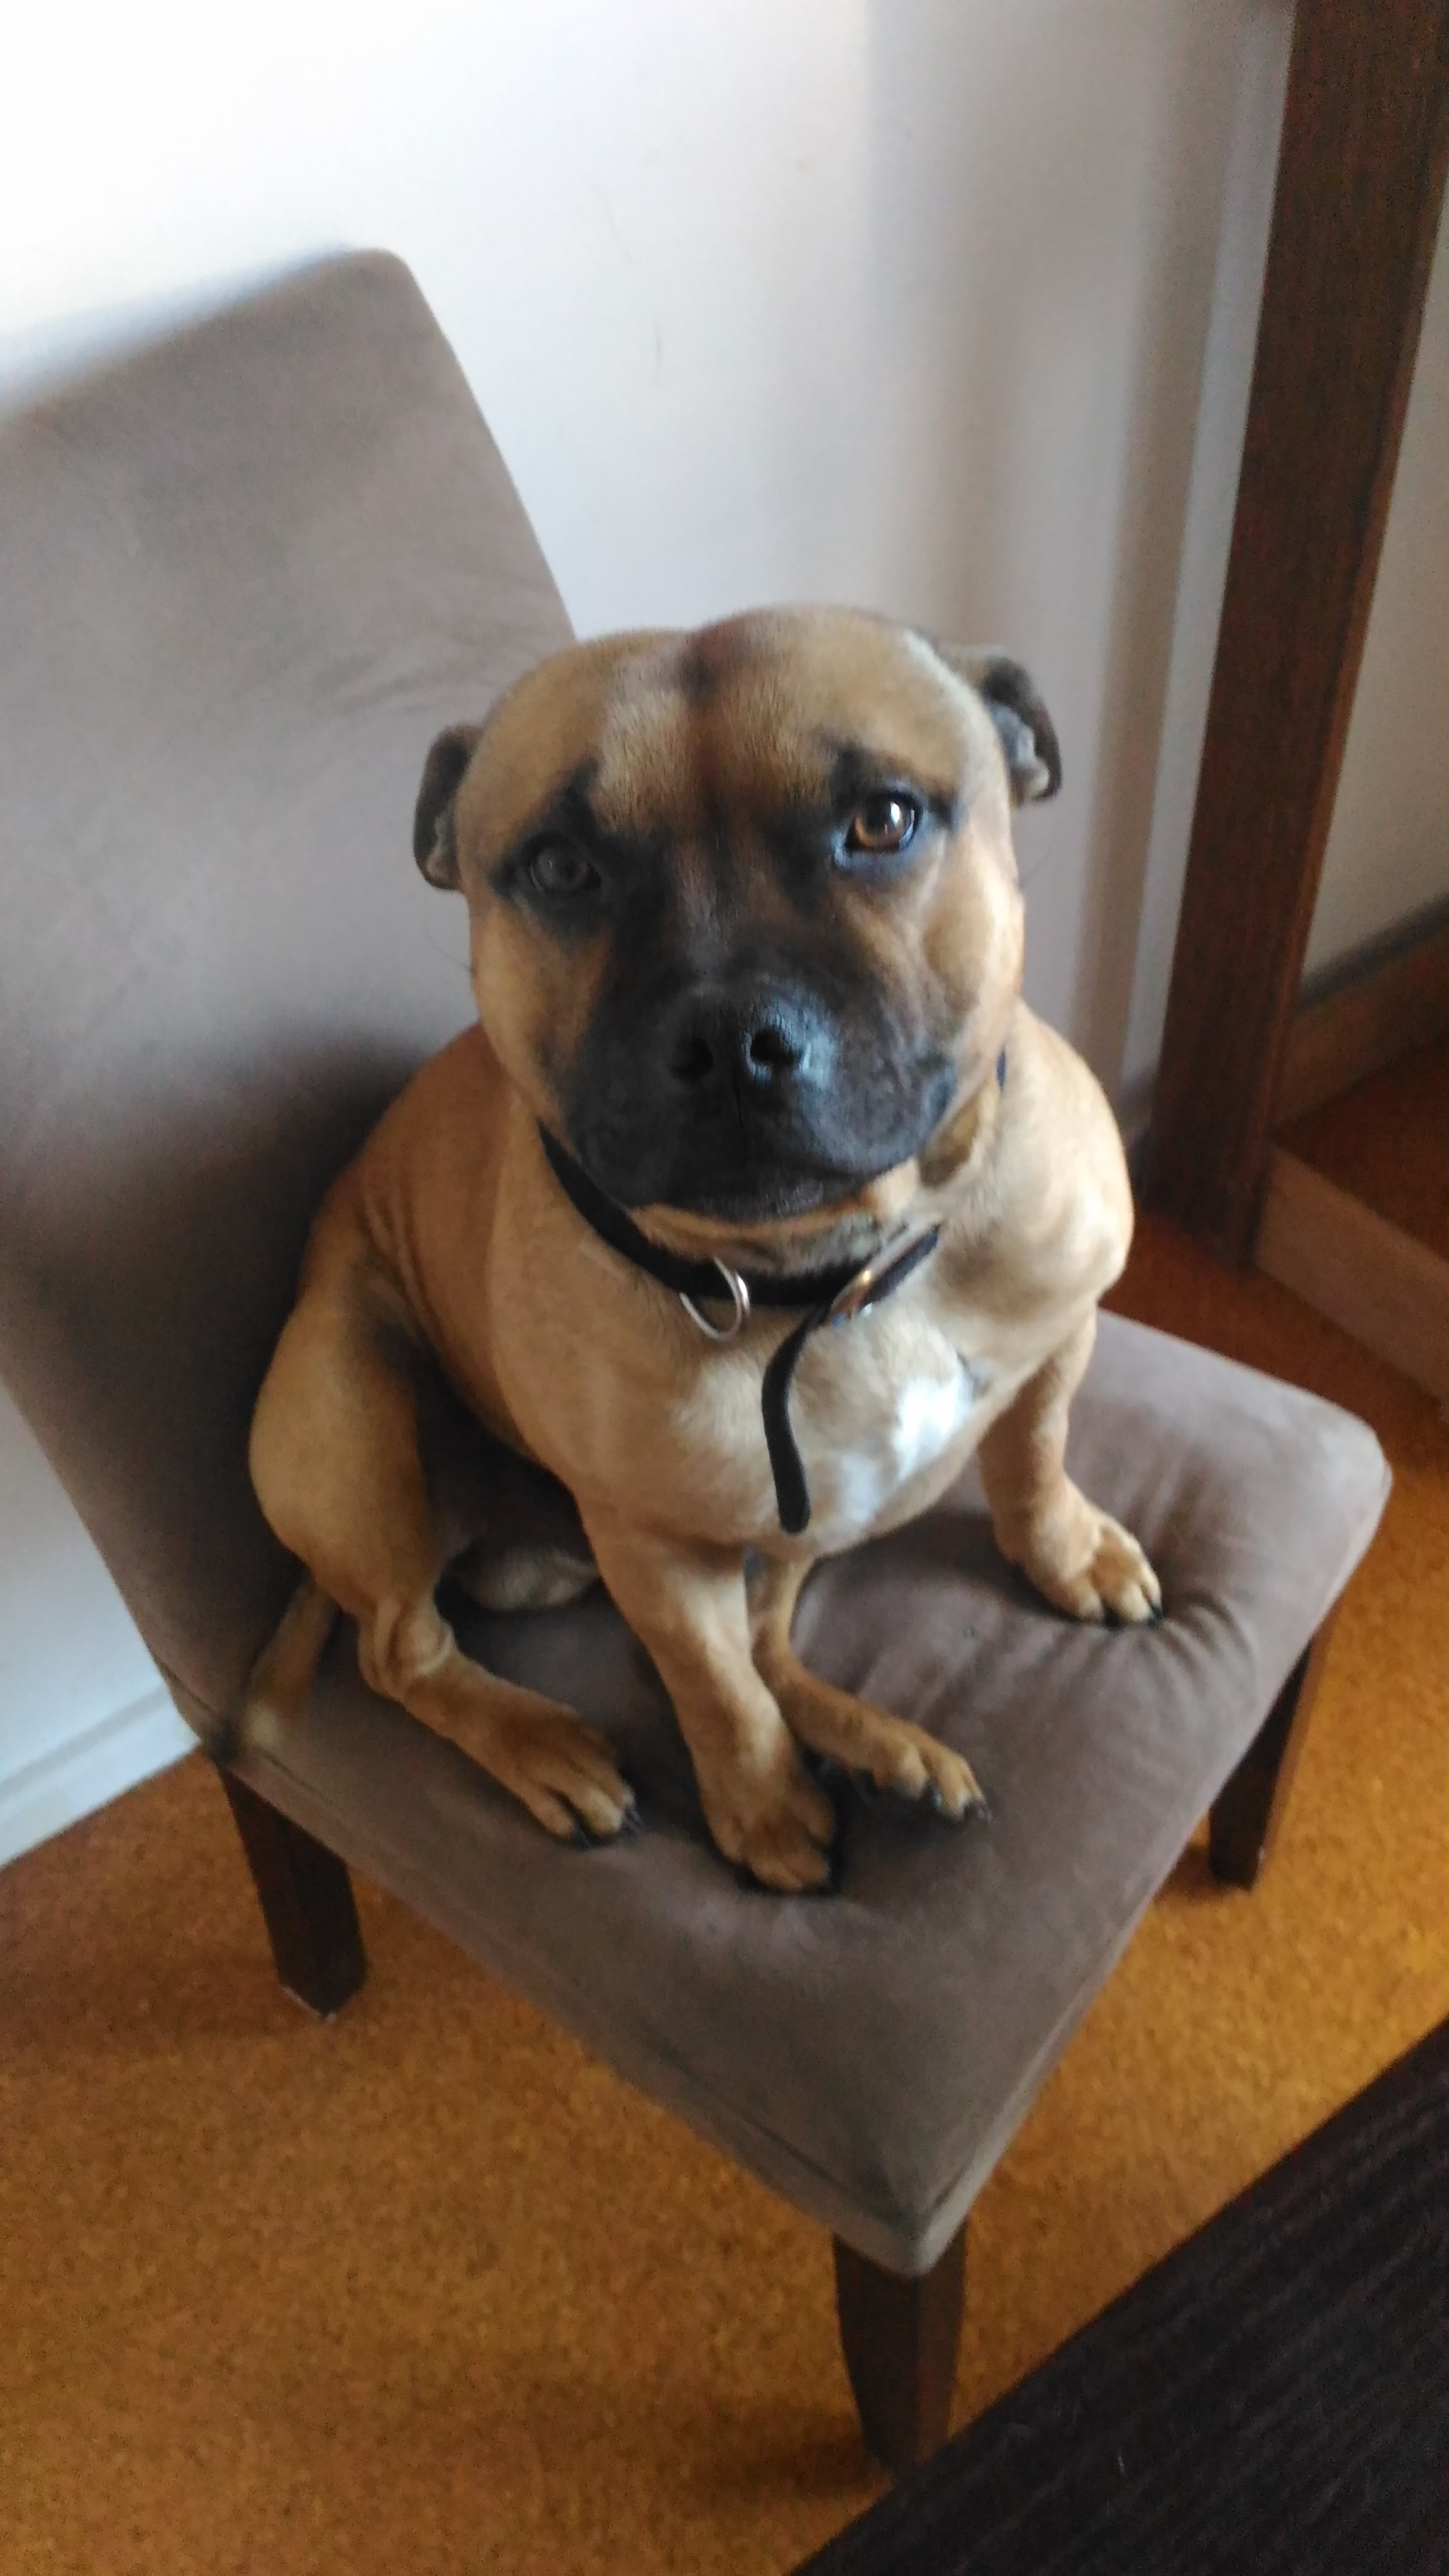
\includegraphics[scale=0.10]{figs/turbo.jpg}


I want to thank Optus, Australian Mobile Service Provider, for unlimited calling hours scheme to India. 
Because of this scheme, I was able to talk to my mom everyday for hours. She is from the generation 
who has seen the mobile and internet revolution in their late age and had hard time coping up with
technological advancement. 
 
  
Some of the great friends who made this journey possible are:
\begin{itemize}
\item Caitlin D'Abrera: 
  She is one the smartest smartest person I know of. She has a super power to break down to problem at finer details 
  to have a better understanding. Moreover, he curiosity to under the tool \textit{git} forced me to learn it properly, 
  so that I can answer her all the queries. Always be curious Caitlin. 
  
 \item Milad Ketabi Ghale Ali: 
   
  \item   Jim De Groot:
  
  \item  Ian Shillito:
  
  \item  Ali Cheraghian
  
  \item Ahmad Attarha
\end{itemize} 


Many thanks to my co-supervisors Rajeev Gor\'e and Michael Norrish. Their valuable feedback during my PhD monitoring 
helped me a lot in shaping my presentation skills. I attended programming language reading group every Wednesday with  Michael, and as usual, 
he was always flawless in explaining ideas. 
 
 I want to thank Thomas Haines, my co-author,  for teaching me all the bits pieces of cryptography. I really 
 enjoyed working with him. 
 
 One of the best experience of this PhD was travelling to Princeton to participate in summer. 
 Unfortunately, I could not attend Marktoberdorf because it was impossible for me to get the visa of Germany, but I hope
 things would be more easier in the upcoming future. 
 
 Last and above all, I want to thank Mina. Being by your side for the last two years has been the best thing that ever happened to me, and I could not 
 imagine life without you.   I am also grateful to all the efforts you made to bear my tendencies to constantly
  talk about set-theory/formal-verification/every-thing-except-romantic.

 Last, but not least, the good wine and beer of Australia could not go unmentioned in this PhD. 
One of the biggest joy of this PhD was to meet my girlfriend, Mina, who came as a visitor to our logic group. 
